%=====================================================================
%  Matrix-Residual Graph Neural Networks for Graph Classification
%  IEEE conference manuscript (IEEEtran, conference option)
%  Target length: 6 pages including references.
%=====================================================================
\documentclass[conference]{IEEEtran}
\IEEEoverridecommandlockouts

\usepackage{cite}
\usepackage{amsmath,amssymb,amsfonts}
\usepackage{graphicx}
\usepackage{textcomp}
\usepackage{xcolor}
\usepackage{booktabs}
\usepackage{array}
\usepackage{url}
\usepackage[hidelinks]{hyperref}

% Tighter float spacing keeps the two-column layout compact.
\setlength{\textfloatsep}{6pt plus 2pt minus 2pt}
\setlength{\floatsep}{6pt plus 2pt minus 2pt}
\setlength{\intextsep}{6pt plus 2pt minus 2pt}
\setlength{\abovecaptionskip}{3pt}
\setlength{\belowcaptionskip}{2pt}
\renewcommand{\arraystretch}{0.92}

% Figures live in two trees: the architecture diagram at the repository root
% and the experiment plots under figures/exp/.
\graphicspath{{../../}{../../figures/}{figures/}}

\begin{document}

\title{Matrix-Residual Graph Neural Networks\\ for Graph Classification}

\author{
\IEEEauthorblockN{Xuelin Hu and Xiaoqin Fu\textsuperscript{*}}
\IEEEauthorblockA{\textit{Liuzhou Railway Vocational Technical College}\\
Liuzhou 545000, China\\
huxuelin@ltzy.edu.cn, fuxiaoqin@ltzy.edu.cn\\
\textsuperscript{*}Corresponding author}
}

\maketitle

\begin{abstract}
Residual connections are widely used to stabilize graph neural networks, yet
residual design is usually treated as a one-dimensional depth-wise choice.
Multi-branch graph classifiers open a richer design space in which residual
information can flow along depth, across branches, or through a local
two-dimensional branch-by-layer neighborhood. This paper studies
Matrix-Residual Graph Neural Networks as a controlled residual-topology
framework for graph classification. The model family represents hidden states
on a branch-by-layer grid and compares five information-flow designs: plain
message passing, vertical residual reuse, horizontal branch-wise exchange,
local matrix residual reuse, and sparse or gated matrix reuse. The main
benchmark evaluates six datasets, four message-passing operators, and five
graph-level folds under a shared training protocol, alongside branch-count
ablations, a mechanism analysis, and a controlled synthetic benchmark spanning
five graph families and two to eight classes. No single residual topology is
universally optimal across datasets and operators, and branch-count ablations
reveal dataset-dependent operating regions rather than monotonic capacity
gains. The synthetic benchmark shows that simple baselines remain competitive
on low-class tasks, whereas matrix residual reuse becomes consistently more
favorable as structural class granularity increases. Residual topology, branch
count, and residual filtering should therefore be selected jointly;
matrix-style reuse is best understood as a tunable residual family rather than
a universal replacement for simpler vertical or horizontal residual paths.
\end{abstract}

\begin{IEEEkeywords}
graph classification, graph neural networks, residual connections,
multi-branch architectures, matrix residual reuse
\end{IEEEkeywords}

\section{Introduction}
\label{sec:intro}

Graph neural networks (GNNs) learn graph representations by repeatedly
aggregating information from local neighborhoods~\cite{kipf2017gcn}.
This message-passing view has become a standard tool for graph classification
because it combines node attributes, local connectivity, and graph-level
structure in a single differentiable model~\cite{gilmer2017neural,wu2020comprehensive}.
Graph classifiers are used well beyond the standard benchmarks, for example to
identify plant vacuole proteins from contact
maps~\cite{suiIdentificationPlantVacuole2023} and to propagate functional
annotation through plant knowledge
graphs~\cite{baongoImprovingPlantFunctional2025}.
In such tasks, graph labels may depend on both local motifs and global
organization, so useful intermediate evidence must survive until graph-level
pooling~\cite{ying2018hierarchical}.

Increasing depth or adding parallel branches expands capacity but also changes
information transport. Deep GNNs may suffer from over-smoothing, where node
representations become too similar across propagation
steps~\cite{li2018deeper,oono2020simple}, or from over-squashing, where
long-range information is compressed into limited-size
messages~\cite{alon2020bottleneck,topping2021understanding}. Both are critical
for graph-level prediction, because the final readout depends on the
intermediate representations that reach the pooling stage. Residual
connections are a common response~\cite{he2016deep,bresson2017residual}, as are
DropEdge and Jumping Knowledge
aggregation~\cite{rong2019dropedge,xu2018representation}. Yet residual
connectivity is usually treated as a default layer-wise component rather than
as the object of study: most residual graph classifiers reuse information along
depth within a single stream.

Once a model contains multiple branches, depth-wise reuse is only one possible
route. Residual information may also move across neighboring branches at the
same depth, or through diagonal branch-depth neighborhoods. Prior work has
strengthened message-passing operators, pooling, and higher-order neighborhood
mixing~\cite{abu2019mixhop,li2024graph}, but
these designs do not isolate the residual-routing question: given several branch
states at a given depth, should the model reuse only the previous state of the
same branch, exchange states laterally, or combine both in a local
two-dimensional neighborhood?

This paper studies residual reuse as a structured design problem on a
branch-by-layer grid. The question is not whether skip connections should exist,
but where residual signals should flow. The grid exposes three controlled
neighborhoods: vertical reuse along depth, horizontal exchange across branches,
and matrix-style reuse combining same-branch, neighboring-branch, and diagonal
paths. A sparse/gated variant tests whether matrix residual traffic should be
filtered before injection. The study is deliberately controlled: the classifier,
readout, fold protocol, and backbone options are held fixed, so that only the
residual topology and its control mechanism vary. Recent models may reach
stronger absolute performance by changing several components at
once~\cite{du2024densegnn}; here those components are intentionally fixed so
that residual topology remains identifiable, following the same discipline as
fair-comparison protocols for graph
classification~\cite{errica2020fair,morris2020tudataset}. Because real
benchmarks span a limited range of structural class granularity, we complement
them with controlled synthetic graph families whose labels are generated by
structural parameters.

The work addresses three research questions. \textbf{RQ1:} Does residual
topology affect performance under a shared graph-classification protocol?
\textbf{RQ2:} How do branch count, residual traffic, and mechanisms explain
performance changes? \textbf{RQ3:} When is matrix-style residual reuse more
effective on real data and on controlled synthetic multi-class structures?

The contributions are:
\begin{itemize}
\item \textbf{A branch-by-layer formulation.} Vertical, horizontal, matrix, and
sparse/gated matrix residual families are expressed as local neighborhoods on
the same grid, making their information-flow differences explicit.
\item \textbf{A controlled real-data and synthetic benchmark.} Classifier,
readout, fold protocol, and backbone choices are matched across all
comparisons, and a structural stress test spans five controlled graph families
and two to eight classes.
\item \textbf{A mechanism analysis with conservative rerun checks.} Accuracy is
analyzed alongside branch diversity, branch cosine similarity, centered kernel
alignment, gradient norms, and residual activity. Sensitivity scans only
identify candidates; selected settings are rerun across folds before being
treated as evidence.
\end{itemize}

\section{Related Work}
\label{sec:related}

\subsection{Message Passing and Expressive Power}

Modern graph learning descends from early recursive models on graph
domains~\cite{gori2005new} and the spectral convolution of
Kipf and Welling~\cite{kipf2017gcn}. GraphSAGE introduced inductive
neighborhood aggregation~\cite{hamilton2017inductive}, graph attention networks
weighted neighbors by learned attention~\cite{velivckovic2017graph}, and the
message-passing neural network framework unified these designs for molecular
property prediction~\cite{gilmer2017neural}. The Weisfeiler--Lehman connection
established by GIN characterizes the discriminative power of this family and
shows that injective multiset aggregation is central to its
expressiveness~\cite{xu2019gin}. Surveys document the resulting design
space~\cite{wu2020comprehensive}, and more recent attention-based
variants extend it further~\cite{sun2023attention}.

\subsection{Deep GNNs and Residual Connectivity}

Depth is not free in message passing. Over-smoothing makes node
representations converge as propagation depth grows~\cite{li2018deeper}, and
this limiting behavior has been analyzed
explicitly~\cite{oono2020simple,chenSimpleDeepGraph2020}. Over-squashing is the
complementary failure mode, in which long-range information is compressed into
fixed-size messages~\cite{alon2020bottleneck,topping2021understanding}. Several
mechanisms target these effects: DropEdge randomly removes edges during
training~\cite{rong2019dropedge}, Jumping Knowledge aggregates representations
across layers~\cite{xu2018representation}, and residual or dense skip paths
carry earlier states forward~\cite{he2016deep,li2019deepgcns,li2021training}.
Residual gated graph convolutional networks learn how strongly historical
states should be reinjected~\cite{bresson2017residual}, and DenseGNN stacks
dense connections for scalable deep
prediction~\cite{du2024densegnn}. These approaches reuse depth-wise state
within a single stream. Our work keeps the same reuse principle but asks a
different question: given several parallel branches, which local residual
neighborhoods on the branch-by-layer grid should be connected.

\subsection{Multi-Branch and Higher-Order Architectures}

Higher-order neighborhood mixing shows that propagating over several hops with
sparsified mixing improves over single-hop
aggregation~\cite{abu2019mixhop}. ARMA filters supply a related frequency-domain
view of multi-hop propagation~\cite{bianchi2020graph}, and graph transformers
generalize attention beyond local
neighborhoods~\cite{dwivedi2020generalization}. Hierarchical pooling adds a
second axis of structure by coarsening graphs as they are
processed~\cite{ying2018hierarchical,lee2019self,cangea2018towards}, and recent
surveys catalogue the resulting
designs~\cite{li2024graph,sun2023attention}. These lines of work increase the
expressive or aggregational capacity of the propagation layer. In contrast, we
hold the propagation operator fixed and vary only how hidden states are reused
across a branch-by-layer grid, so that the residual topology itself becomes the
identifiable factor.

\subsection{Controlled Evaluation for Graph Classification}

Because graph benchmarks are sensitive to splitting, feature choice, and
operator tuning, careful comparative protocols matter. Errica \emph{et al.}
argue for matched evaluation conditions when comparing graph
classifiers~\cite{errica2020fair}, and TUDataset provides the standardized
collection on which much of this evaluation
rests~\cite{morris2020tudataset}. We follow the same discipline: the readout,
optimizer schedule, fold partition, and backbone options are matched across the
compared residual families, and only the residual neighborhood and
residual-control mechanism change.

\section{Method}
\label{sec:method}

\subsection{Notation and Shared Pipeline}
\label{sec:pipeline}

Let \(\mathcal{G}=(\mathcal{V},\mathcal{E})\) be a graph with node feature
matrix \(\mathbf{X}\in\mathbb{R}^{n\times d_{\mathrm{in}}}\) and adjacency
structure \(\mathbf{A}\). Given a dataset
\(\mathcal{D}=\{(\mathcal{G}_i,y_i)\}_{i=1}^{N}\), the objective is to learn
\(f_{\theta}:\mathcal{G}\rightarrow \hat{y}\), where \(\hat{y}\) is the predicted
graph label. Let \(B\) be the number of branches and \(L\) the number of
message-passing layers, and write the hidden state at branch \(b\) and layer
\(\ell\) as \(\mathbf{H}^{(\ell)}_{b}\), with \(b\in\{1,\ldots,B\}\). A
branch-local propagation step is
\begin{equation}
\mathbf{Z}^{(\ell)}_{b} =
\phi^{(\ell)}_{b}\left(\mathbf{H}^{(\ell-1)}_{b}, \mathbf{A}\right),
\label{eq:prop}
\end{equation}
where \(\phi\) is one of four standard operators: GCNConv \cite{kipf2017gcn},
GATConv \cite{velivckovic2017graph}, SAGEConv \cite{hamilton2017inductive}, or
GINConv \cite{xu2019gin}. The residual-enhanced update is
\begin{equation}
\mathbf{H}^{(\ell)}_{b} =
\mathbf{Z}^{(\ell)}_{b} +
\sum_{(b',\ell')\in\mathcal{N}(b,\ell)}
\mathcal{R}_{(b',\ell')\rightarrow(b,\ell)}
\left(\mathbf{H}^{(\ell')}_{b'}\right).
\label{eq:update}
\end{equation}
Only the residual neighborhood \(\mathcal{N}(b,\ell)\) and the residual
transform \(\mathcal{R}\) change across architectures. After the final layer,
each branch is pooled to a graph-level vector by global mean pooling, and the
branch vectors are combined before classification with a cross-entropy loss. We
deliberately avoid architecture-specific pooling heads such as differentiable
pooling~\cite{ying2018hierarchical}, because the goal is to isolate residual
topology rather than to compare readout mechanisms.
Fig.~\ref{fig:architecture} summarizes the shared pipeline and the compared
residual routes. The four operators were chosen as canonical representatives of
spectral-style convolution, attention-based aggregation, neighborhood sampling
and aggregation, and injective multiset aggregation.

\begin{figure}[!t]
\centering
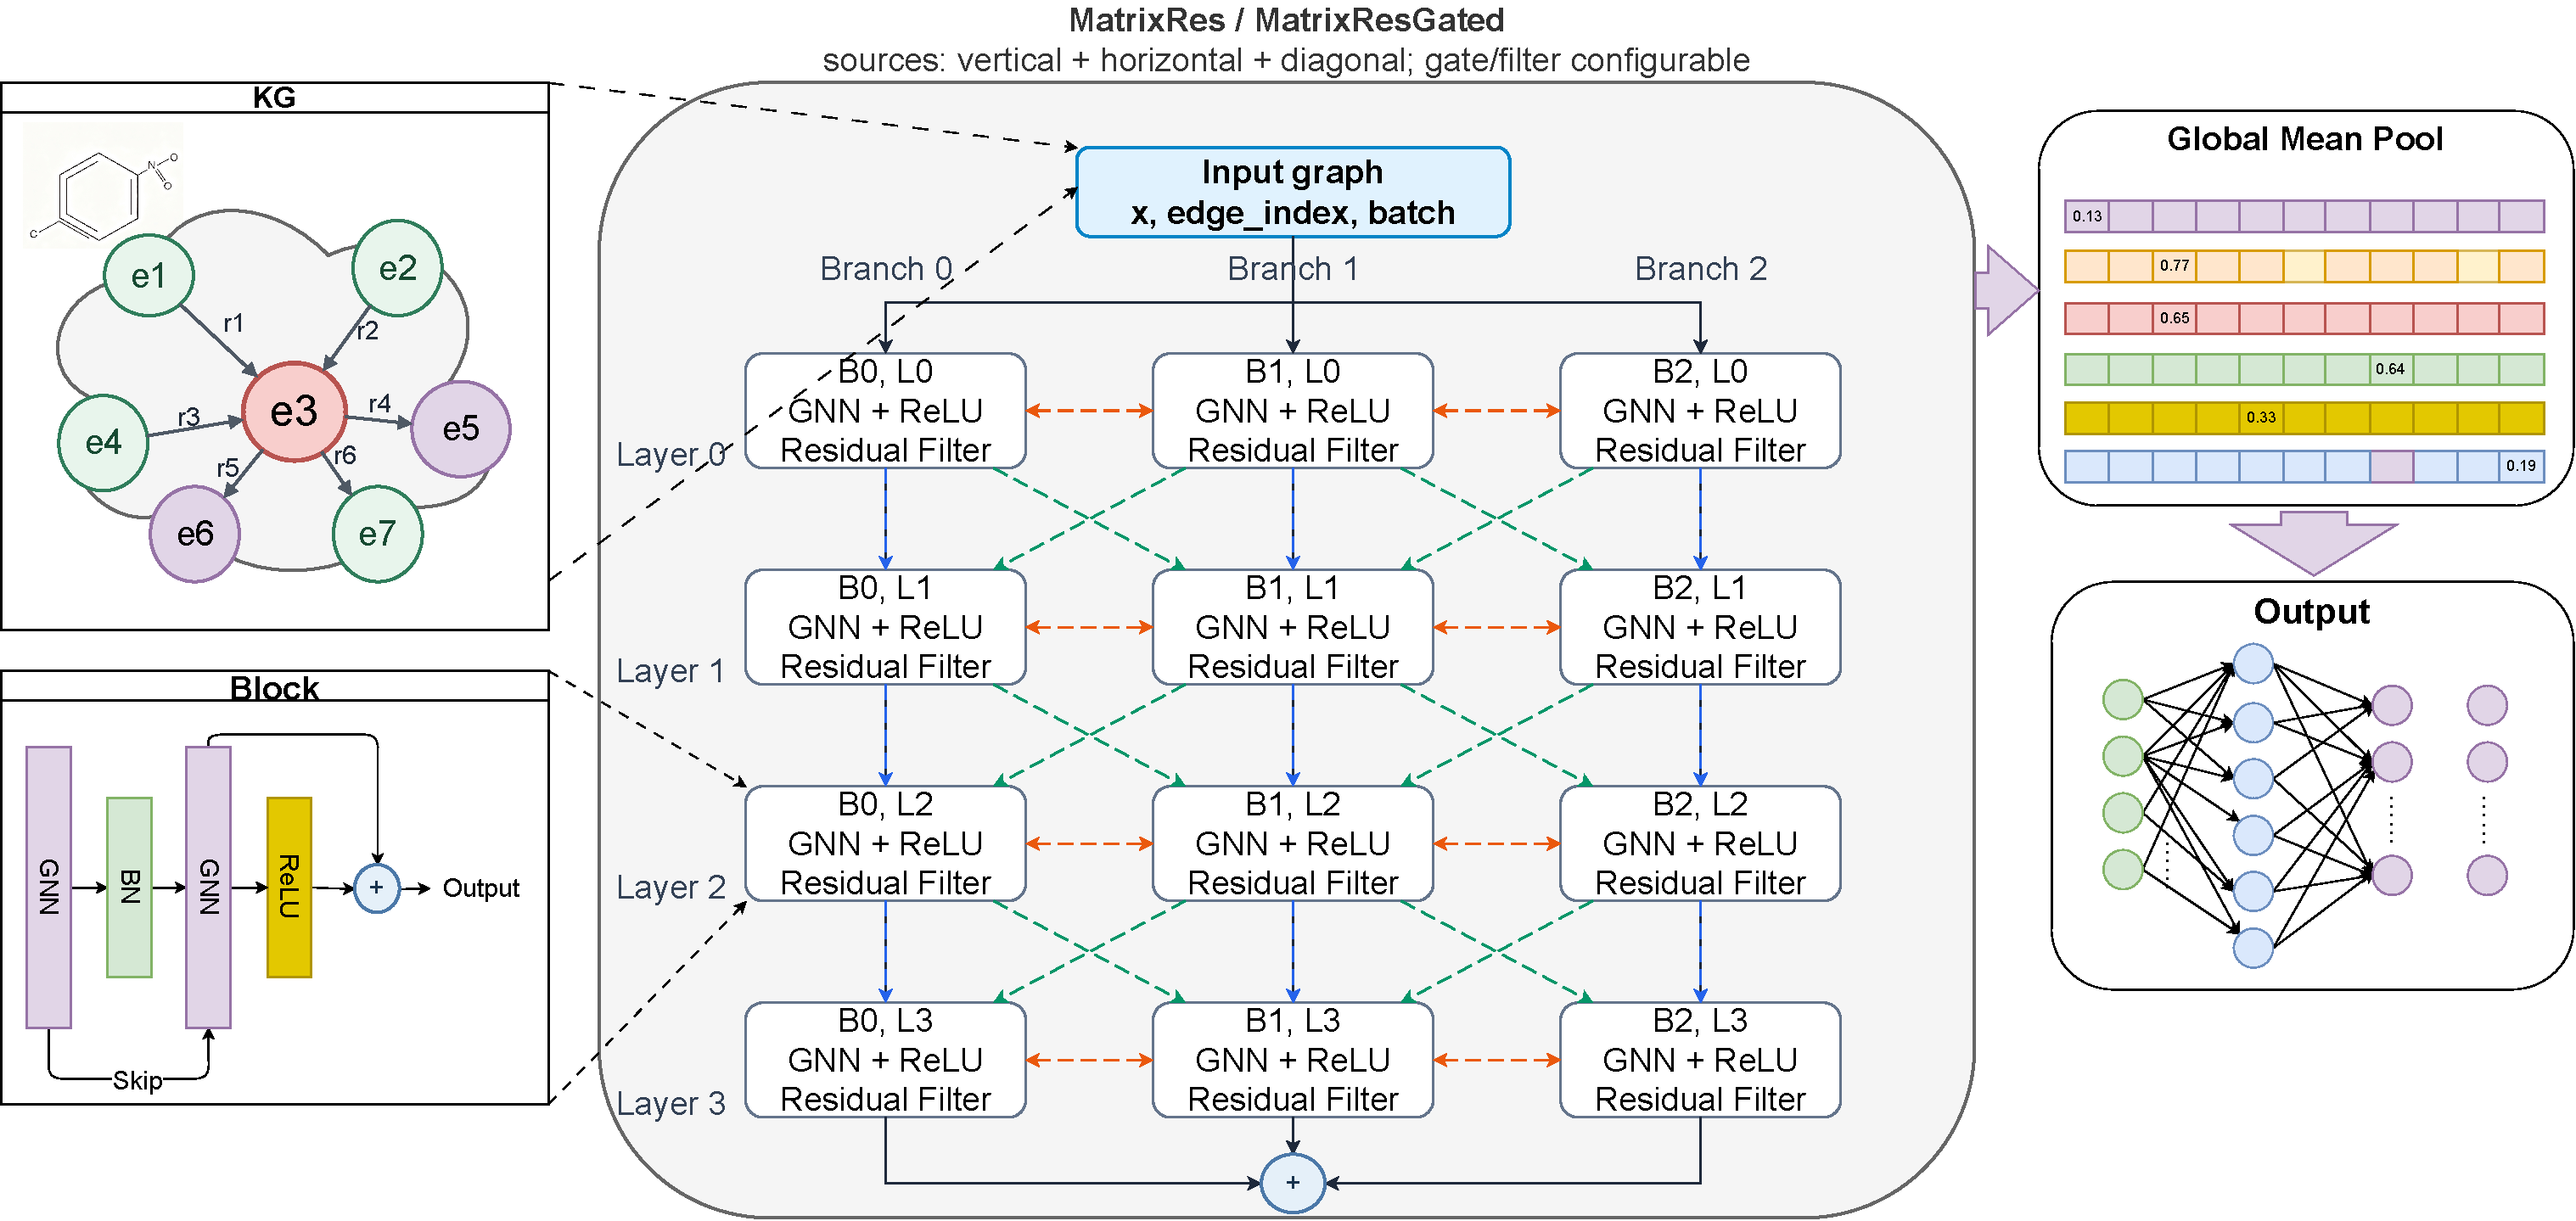
\includegraphics[width=0.95\columnwidth]{figures/cr_gnn_graph_architecture.pdf}
\caption{Compared residual neighborhoods on the branch-by-layer grid; the
backbone and graph-level readout are held fixed while the residual routes
change.}
\label{fig:architecture}
\end{figure}

\subsection{Residual Neighborhoods}
\label{sec:model}

\textbf{Plain} has no residual neighborhood, \(\mathcal{N}(b,\ell)=\emptyset\).
\textbf{VerticalRes} injects the previous layer of the same branch,
\(\mathcal{N}(b,\ell)=\{(b,\ell-1)\}\). \textbf{HorizontalRes} exchanges
information across adjacent branches at the same depth,
\(\mathcal{N}(b,\ell)=\{(b-1,\ell),(b+1,\ell)\}\), with boundary branches using
only valid neighbors; when \(B=1\) this neighborhood is empty. \textbf{MatrixRes}
combines vertical, horizontal, and diagonal neighbors:
\begin{equation}
\mathcal{N}(b,\ell)=
\{(b,\ell-1),(b-1,\ell),(b+1,\ell),(b-1,\ell-1),(b+1,\ell-1)\}.
\label{eq:matrix}
\end{equation}
This local stencil is intentionally not dense all-to-all mixing: it preserves an
interpretable residual structure over the branch-by-layer grid. Invalid boundary
neighbors are removed, so when \(B=1\), MatrixRes keeps the same-branch vertical
path after the first layer but has no branch-neighbor routes.

\textbf{MatrixResGated} uses the same neighborhood but controls the injected
signal through the residual transform:
\begin{equation}
\mathcal{R}(\mathbf{U}) =
\begin{cases}
\alpha \mathbf{U}, & \text{identity filtering with a gate},\\[2pt]
\alpha\,\mathrm{softshrink}_{\lambda}(\mathbf{U}), & \text{sparse filtering with a gate}.
\end{cases}
\label{eq:gate}
\end{equation}
Plain, VerticalRes, HorizontalRes, and MatrixRes use identity residual
filtering. MatrixResGated uses sparse filtering with \(\lambda=0.05\) and a
learnable scalar gate initialized at 0.8; when \(B=1\) it still applies gated
sparse filtering to the remaining matrix-residual paths. Top-\(k\) filtering and
fixed gates are supported but are not used for the reported results.

\subsection{Experimental Setup}
\label{sec:setup}

The main benchmark uses six TUDataset collections~\cite{morris2020tudataset}
accessed through PyTorch Geometric~\cite{fey2019fast}: PROTEINS, DD, ENZYMES,
MUTAG, AIDS, and Mutagenicity. PROTEINS and DD are binary protein-structure
tasks, ENZYMES is six-class, and MUTAG, AIDS, and Mutagenicity provide
molecular-graph robustness checks. Graphs are loaded with their provided
features; no handcrafted descriptors, augmentation, or edge rewiring are used,
so that the comparison reflects residual topology rather than feature
engineering.

All results use graph-level five-fold evaluation. For fold \(k\), test accuracy
is \(\mathrm{Acc}_{k}=|\mathcal{T}_{k}|^{-1}\sum_{(\mathcal{G}_{i},y_{i})\in\mathcal{T}_{k}}
\mathbf{1}[\hat{y}_{i}=y_{i}]\), and we report the mean over folds together with
the fold-level standard deviation. Accuracy is the primary metric because every
benchmark has discrete graph labels. For the synthetic benchmark we additionally
report macro-F1, which weights each class equally, and chance-normalized
accuracy, \(\mathrm{NAcc}=(\mathrm{Acc}-1/C)/(1-1/C)\), because raw accuracy is
not comparable across class counts. Mechanism metrics such as branch diversity,
cosine similarity, centered kernel alignment (CKA), residual activity, and
gradient norm are used as diagnostics, not as optimization targets.

To test residual topology under controlled structural granularity we add a
synthetic benchmark over five graph families: Bernoulli random graphs (ER),
Barab\'asi--Albert (BA) graphs, stochastic block models
(SBM)~\cite{holland1983stochastic}, Watts--Strogatz (WS)
graphs~\cite{watts1998collective}, and a regular-degree control. For each family
we generate seven datasets with \(C\in\{2,\ldots,8\}\) classes, 200 graphs per
class, and 30--80 nodes per graph. Node features are eight-dimensional vectors
derived from normalized degree and random channels; they do not encode the
label. Labels are controlled by family-specific structural parameters: edge
probability for ER~\cite{gilbert1959random}, preferential-attachment count for
BA~\cite{barabasi1999emergence}, within- and between-block probabilities for
SBM, rewiring probability for WS, and fixed degree for the regular control.
These families serve as stress tests, not as replacements for real benchmarks.

Table~\ref{tab:hyperparams} lists the shared settings. Models are optimized with
Adam~\cite{kingma2014adam}, and the checkpoint with the lowest validation loss
is retained for test evaluation.
Branch-count ablations
evaluate \(B=1,\ldots,8\) for HorizontalRes, MatrixRes, and MatrixResGated on
PROTEINS and DD under GCNConv. Sensitivity scans run on fold 0 at \(B=3\),
varying learning rate, dropout, hidden dimension, sparsity strength, and gate
initialization; selected candidates are then rerun across all five folds.
Experiments ran on an Ubuntu server with an AMD Ryzen 7 5700X CPU and an NVIDIA
RTX 3090 GPU.

\begin{table}[!t]
\centering
\caption{Key Experimental Settings}
\label{tab:hyperparams}
\footnotesize
\begin{tabular}{@{}p{0.38\columnwidth}p{0.58\columnwidth}@{}}
\toprule
Parameter & Value \\
\midrule
Operators & GCNConv, GATConv, SAGEConv, GINConv \\
Branches / layers & \(B=3\); \(L=4\) (DD: \(L=3\)) \\
Hidden dimension & 64 \\
Evaluation & Five-fold graph classification \\
Plain/Vertical/Horizontal & 200 epochs, patience 60, lr 0.005, wd \(10^{-4}\), dropout 0.5 \\
MatrixRes/MatrixResGated & 240 epochs, patience 80, lr 0.003, wd \(5\times10^{-5}\), dropout 0.3 \\
Schedule & ReduceLROnPlateau, factor 0.5, patience 15, min lr \(10^{-5}\) \\
Gradient clipping & Norm 2.0 \\
\bottomrule
\end{tabular}
\end{table}

\section{Results}
\label{sec:results}

All results are five-fold mean best test accuracy \(\pm\) fold-level standard
deviation unless stated otherwise.

\subsection{Overall Benchmark}
\label{sec:res-overall}

The main benchmark asks whether residual topology has a stable winner across
datasets and operators. It does not. Across the 24 dataset--operator
combinations (Table~\ref{tab:operator_wins}), MatrixRes is the most frequent
winner with 9 wins and the best mean rank (2.12); MatrixResGated and Plain win 5
combinations each, HorizontalRes wins 3, and VerticalRes wins 2. Matrix-style
reuse therefore has the most favorable aggregate profile, but every topology is
strongest in some setting. The per-dataset winners are mixed: the matrix family
dominates MUTAG, AIDS, and Mutagenicity, whereas PROTEINS alternates between
Plain and HorizontalRes and DD alternates among HorizontalRes, MatrixRes, and
VerticalRes. ENZYMES remains difficult and shows no stable preference.

\begin{table}[!t]
\centering
\caption{Winner Counts and Mean Ranks over the 24 Dataset--Operator
Combinations}
\label{tab:operator_wins}
\footnotesize
\begin{tabular}{@{}lccc@{}}
\toprule
Model & Wins & Mean rank & \multicolumn{1}{l}{GCNConv wins} \\
\midrule
Plain          & 5 & 3.04 & PROTEINS \\
VerticalRes    & 2 & 3.38 & --- \\
HorizontalRes  & 3 & 3.54 & DD \\
MatrixRes      & \textbf{9} & \textbf{2.12} & MUTAG, AIDS, Mutagenicity \\
MatrixResGated & 5 & 2.92 & ENZYMES \\
\bottomrule
\end{tabular}
\end{table}

ENZYMES should be read cautiously, because the absolute accuracies are low for
all models. Excluding it leaves MatrixRes with 9 wins over 20 combinations and a
mean rank of 2.05, so the aggregate preference is unchanged.

To remove variation caused by the operator, we also report the GCNConv slice
separately (Table~\ref{tab:main_benchmark}, Fig.~\ref{fig:main_benchmark}). The
same conclusion holds: MatrixRes is the strongest choice on MUTAG, AIDS, and
Mutagenicity, while simpler residual paths remain preferable on PROTEINS, DD,
and ENZYMES. Residual topology matters, but its value depends on the dataset.

\begin{table}[!t]
\centering
\caption{GCNConv Benchmark at \(B=3\) (Mean \(\pm\) Std. over Five Folds)}
\label{tab:main_benchmark}
\footnotesize
\begin{tabular}{@{}lccccc@{}}
\toprule
Dataset & Plain & Vertical & Horizontal & Matrix & MatrixGated \\
\midrule
PROTEINS     & \(\mathbf{0.7044}\) & 0.6993 & 0.6992 & 0.6973 & 0.6886 \\
DD           & 0.7053 & 0.7143 & \(\mathbf{0.7181}\) & 0.7127 & 0.7141 \\
ENZYMES      & 0.2683 & 0.2550 & 0.2633 & 0.2750 & \(\mathbf{0.2933}\) \\
MUTAG        & 0.7556 & 0.7451 & 0.7343 & \(\mathbf{0.7609}\) & 0.7556 \\
AIDS         & 0.8215 & 0.8210 & 0.8130 & \(\mathbf{0.8365}\) & 0.8150 \\
Mutagenicity & 0.7644 & 0.7667 & 0.7738 & \(\mathbf{0.7784}\) & 0.7701 \\
\bottomrule
\end{tabular}
\end{table}

\begin{figure}[!t]
\centering
\includegraphics[width=0.98\columnwidth]{figures/exp/fig_main_benchmark_gcnconv.pdf}
\caption{GCNConv benchmark at \(B=3\). Fold-level standard deviations range
from 0.005 to 0.072 across cells.}
\label{fig:main_benchmark}
\end{figure}

\subsection{Synthetic Multi-Class Scaling}
\label{sec:res-synthetic}

The synthetic benchmark asks whether residual topology behaves differently as
structural class granularity increases under controlled graph-generation rules.
Table~\ref{tab:synthetic_class_scaling} summarizes the trend averaged over the
five families and four operators. Low-class settings do not favour matrix-style
reuse: Plain is best at \(C=2\) and HorizontalRes at \(C=3\). From \(C=4\)
onward matrix-style reuse becomes more competitive, and MatrixResGated is the
strongest mean-accuracy model at \(C=4\), \(C=5\), \(C=6\), and \(C=8\). Over the
higher-class regime \(C=4,\ldots,8\), MatrixResGated reaches 0.6943 accuracy and
0.6324 normalized accuracy against 0.6827 and 0.6183 for Plain, while MatrixRes
has the best macro-F1 (0.6880). MatrixRes also degrades least from \(C=2\) to
\(C=8\) (0.3479 points, against 0.3720 for Plain), suggesting that dense local
matrix reuse is relatively stable as the label space becomes finer.

\begin{table}[!t]
\centering
\caption{Synthetic Scaling Averaged over Five Graph Families and Four
Operators}
\label{tab:synthetic_class_scaling}
\footnotesize
\begin{tabular}{@{}clcccc@{}}
\toprule
Classes & Best model & Plain & Matrix & MatrixGated & Best NAcc \\
\midrule
2 & Plain          & \(\mathbf{0.9585}\) & 0.9481 & 0.9578 & 0.9170 \\
3 & HorizontalRes  & 0.8774 & 0.8600 & 0.8772 & 0.8200 \\
4 & MatrixResGated & 0.8002 & 0.8083 & \(\mathbf{0.8111}\) & 0.7481 \\
5 & MatrixResGated & 0.7233 & 0.7280 & \(\mathbf{0.7296}\) & 0.6621 \\
6 & MatrixResGated & 0.6719 & 0.6827 & \(\mathbf{0.6878}\) & 0.6254 \\
7 & VerticalRes    & 0.6314 & 0.6429 & 0.6395 & 0.5945 \\
8 & MatrixResGated & 0.5865 & 0.6002 & \(\mathbf{0.6035}\) & 0.5469 \\
\bottomrule
\end{tabular}
\end{table}

\begin{figure}[!t]
\centering
\includegraphics[width=0.98\columnwidth]{figures/exp/fig_synthetic_multiclass_scaling.pdf}
\caption{Synthetic scaling from two to eight classes, averaged over five graph
families and four operators.}
\label{fig:synthetic_multiclass_scaling}
\end{figure}

At the family level, MatrixRes is strongest in the higher-class BA, ER, and
regular-degree settings, where labels are tied to degree growth, edge
probability, or degree-uniform structural change. These families share a
pattern: the label space is formed by related structural regimes rather than
unrelated categories, so local matrix reuse can combine depth-wise refinement
with neighboring-branch exchange. SBM is community-driven and less favourable
to matrix-style reuse, though MatrixRes remains close to the best result.

\subsection{Branch-Count Ablation and Mechanism Analysis}
\label{sec:res-branch}

Branch count is not merely a capacity parameter, because it also changes
residual-path density. Table~\ref{tab:branch_best} reports the best and worst
branch counts per topology. On PROTEINS the useful region is moderate
(HorizontalRes peaks at \(B=4\), MatrixRes at \(B=6\), MatrixResGated at
\(B=3\)); on DD it is smaller (HorizontalRes and MatrixRes peak at \(B=2\),
MatrixResGated is strongest already at \(B=1\)). Branch expansion is therefore
not monotonic and must be matched to task structure.

\begin{table}[!t]
\centering
\caption{Branch-Count Ablation: Best and Worst Settings}
\label{tab:branch_best}
\footnotesize
\begin{tabular}{@{}llcccc@{}}
\toprule
Dataset & Model & Best \(B\) & Best acc. & Worst \(B\) & Worst acc. \\
\midrule
PROTEINS & HorizontalRes  & 4 & \(\mathbf{0.7125}\) & 1 & 0.6801 \\
PROTEINS & MatrixRes      & 6 & \(\mathbf{0.7062}\) & 1 & 0.6909 \\
PROTEINS & MatrixResGated & 3 & \(\mathbf{0.7098}\) & 4 & 0.6711 \\
DD       & HorizontalRes  & 2 & \(\mathbf{0.7275}\) & 4 & 0.7071 \\
DD       & MatrixRes      & 2 & \(\mathbf{0.7206}\) & 7 & 0.7071 \\
DD       & MatrixResGated & 1 & \(\mathbf{0.7283}\) & 7 & 0.7053 \\
\bottomrule
\end{tabular}
\end{table}

\begin{figure}[!t]
\centering
\includegraphics[width=0.98\columnwidth]{figures/exp/fig_branch_count_ablation.pdf}
\caption{Branch-count ablation on PROTEINS and DD under GCNConv. Accuracy rises
only within an effective operating region before saturating or declining.}
\label{fig:branch_ablation}
\end{figure}

The mechanism metrics explain this split. On PROTEINS, HorizontalRes improves
from \(B=1\) to \(B=4\) while branch diversity rises from 0.0000 to 1.1450 and
branch cosine falls from 1.0000 to 0.8417, but diversity alone is not sufficient:
at \(B=8\) diversity increases further to 1.5441 while accuracy drops to 0.6881.
MatrixRes follows the same pattern at a larger scale, peaking at \(B=6\) with a
diversity of 3.7755. On DD the best settings have nearly saturated branch cosine
(0.9969 for HorizontalRes and 0.9991 for MatrixRes at \(B=2\)) and CKA of
1.0000, so extra residual traffic is unlikely to create new functional
separation; larger branch counts raise diversity without improving accuracy.
MatrixResGated behaves as genuine residual control rather than a dense path: its
active ratio is 0.3121 at the best PROTEINS setting and 0.2352 at the best DD
setting, while the learned gate stays near 0.78--0.84 rather than collapsing.
These are diagnostic correlations rather than causal interventions. The gated
variant does not dominate MatrixRes overall, so sparse filtering is best treated
as a traffic-control mechanism, not a universal improvement.

\subsection{Sensitivity and Five-Fold Validation}
\label{sec:res-sensitivity}

Fold-0 scans only identify candidates. On PROTEINS, MatrixRes does not improve
over its fold-0 baseline in the tested sweep, while MatrixResGated has a
mild-sparsity candidate (\(\lambda=0.02\) raises fold-0 accuracy from 0.6726 to
0.6951; stronger sparsification is harmful). On DD both models prefer lighter
hidden dimensions, reaching 0.7595 and 0.7511 at \(d=32\). Rerunning selected
candidates across all five folds prevents over-claiming: on DD the \(d=32\)
MatrixResGated candidate stays competitive at \(0.7215\pm0.0330\) while cutting
parameters from 42{,}371 to 15{,}043, whereas on PROTEINS the sparsity candidate
does not preserve its fold-0 advantage (\(0.6909\pm0.0447\)) and remains
unstable rather than a confirmed gain.

\section{Discussion}
\label{sec:discussion}

\subsection{RQ1: Residual Topology and Performance}
\label{sec:rq1}

The main benchmark argues against a universal residual topology: MatrixRes is
the most frequent winner with the best mean rank, but all five model families
win at least two of the 24 dataset--operator combinations, and the GCNConv slice
also has dataset-dependent winners. The useful residual neighborhood therefore
depends on dataset-specific tolerance for branch specialization, residual
traffic, and optimization complexity. This is consistent with the broader
literature, where changing the propagation operator, normalization, or pooling
design shifts the preferred
architecture~\cite{xu2019gin,hamilton2017inductive,ying2018hierarchical}. The
present study adds residual topology itself as another source of that shift.
Matrix-style reuse can be read as a local residual stencil over the
branch-by-layer grid, analogous in spirit to structured neighborhood
mixing~\cite{abu2019mixhop} but applied to hidden-state reuse rather than graph
adjacency; its advantage is architectural organization, not a new
message-passing primitive.

\subsection{RQ2: Branch Count and Mechanisms}
\label{sec:rq2}

Increasing \(B\) adds branches, residual paths, and optimization interactions at
once, so it is not a simple capacity knob. PROTEINS tolerates a moderate budget
(peaks at \(B=4\)--\(6\)) whereas DD prefers \(B=1\)--\(2\). The mechanism
metrics are consistent with this split: on PROTEINS the best settings combine
increased branch diversity with reduced branch cosine, while on DD the best
settings have nearly saturated cosine and CKA, so additional residual traffic is
unlikely to create new functions. Diversity may rise with \(B\) but does not by
itself improve classification when branch similarity stays high or gradients
weaken. This rise-then-fall behaviour is a practical warning for residual GNN
design, since residual connections are often introduced to make deeper or wider
models easier to optimize~\cite{he2016deep}. The balance between
functional diversity and residual interference differs sharply between two
datasets that are both routinely treated as protein-structure benchmarks.

\subsection{RQ3: When Matrix-Style Reuse Helps}
\label{sec:rq3}

Sparse/gated reuse is not uniformly better than dense matrix reuse: MatrixRes
wins more combinations overall. MatrixResGated remains useful as a controlled
way to suppress weak residual coefficients, and the mechanism table confirms
that it keeps fewer active pathways than dense MatrixRes while the gate stays at
a moderate value. Its value is not that sparsity always improves accuracy, but
that filtering helps when matrix reuse would otherwise inject too much
low-value traffic. This places it between two familiar ideas: like residual
gated graph networks it learns how strongly historical information should be
injected~\cite{bresson2017residual}, and like sparsification methods it reduces
the influence of weak pathways~\cite{rong2019dropedge}. The implementation is
deliberately simple---a scalar gate and soft-shrink filtering rather than a
large routing network---which keeps the ablation interpretable. Candidate
settings must still be validated across folds: the DD hidden-dimension candidate
survives that check and yields a smaller, more efficient model, whereas the
PROTEINS sparsity candidate does not and should not be claimed as a gain.

The synthetic benchmark separates class granularity from real-dataset
idiosyncrasies. Simple residual choices remain competitive at two and three
classes, which guards against the overbroad claim that matrix-style reuse is
always needed. From four classes onward the pattern reverses: MatrixResGated has
the best average and normalized accuracy, MatrixRes has the best macro-F1 and
the smallest degradation from \(C=2\) to \(C=8\). Distribution-level results
refine this: MatrixRes leads in the degree- and density-driven BA, ER, and
regular-degree families, whose labels separate related structural regimes rather
than unrelated categories, while community-driven SBM is less favourable. Taken
together, matrix-style reuse is conditionally effective rather than universal,
and is most useful when the task requires separating several related structural
regimes under finer discrimination.

\subsection{Limitations}
\label{sec:limitations}

Several factors bound these findings. The benchmark uses a fixed graph-level
pooling and classification head, so alternative readouts may interact with
residual topology. The compared operators are canonical message-passing
backbones rather than recent graph transformers or local-global
hybrids~\cite{dwivedi2020generalization}, which is a deliberate control choice
but means the study is not a state-of-the-art comparison. The sensitivity scan is fold-0 only, and the candidate reruns cover
MatrixResGated on PROTEINS and DD alone. ENZYMES has low absolute accuracy and
high variability. The mechanism analysis is correlational: branch diversity,
cosine similarity, CKA, and gradient norms support a coherent explanation but do
not prove causality. Finally, the benchmark intentionally avoids task-specific
chemical or biological feature engineering, so absolute accuracies should not be
read as optimized state-of-the-art molecular prediction results, and the
synthetic families stress-test residual topology rather than substitute for
broader real multi-class benchmarks. Future work should extend the comparison to
larger datasets, richer readouts, recent local-global backbones, and learned
residual-neighborhood policies that replace the hand-specified vertical,
horizontal, and matrix stencils.

\section{Conclusion}
\label{sec:conclusion}

This paper studied residual connectivity for graph classification as a
structured branch-by-layer design problem. Across six datasets and four
message-passing operators, residual topology matters, but its value depends on
the dataset, operator, and branch budget. MatrixRes is the most frequent winner
with the best mean rank in the full benchmark, yet the per-dataset GCNConv
winners remain mixed, and ENZYMES has low absolute accuracy and should be read
cautiously. Branch-count ablations show that adding branches helps only within a
limited operating region: additional branches raise representational diversity
but also residual traffic, and they can preserve redundant branch similarity or
weaken optimization. The synthetic multi-class benchmark supports a conditional
reading---matrix-style reuse is unnecessary for the easiest two- and three-class
settings but becomes more competitive from four classes onward, where
MatrixResGated attains the best average and normalized accuracy and MatrixRes
degrades least from two to eight classes. The practical implication is that
residual topology, branch count, operator choice, and residual control should be
evaluated jointly, and that candidate settings should be rerun across folds
before a sensitivity result is treated as a performance claim.

\section*{Acknowledgment}

This work was supported by the Science and Technology Research Project of Henan
Province (Grant No.~262102211055) and the Key Scientific Research Project of
Colleges and Universities in Henan Province (Grant No.~27AQ520018). The authors
thank the reviewers and editors for their time and feedback.

\section*{Data Availability}

The code and experiment records supporting this study are available from the
corresponding author on reasonable request.


\bibliographystyle{IEEEtran}
\bibliography{references}

\end{document}
